\section{Bias in Data}
Since data plays an important role in the outcome of the model and can directly affect the fairness constraints if it contains any biases, we decided to analyze some of the datasets that are widely used in the training of NER models to determine whether they show any biases toward a specific group that could result in the biased behavior observed in those results discussed in previous sections. 
\begin{table}
\begin{tabular}{ p{2.6cm}p{1.4cm}p{2.4cm}}
 \toprule
 Female Name&Frequency&Error Type\\
 \midrule
 Charlotte&12,940&Tagged as LOC\\[0.5pt]
 Sofia&7,621&Tagged as LOC\\[0.5pt]
 Victoria&7,089&Tagged as LOC\\[0.5pt]
 Madison&7,036&Tagged as LOC\\[0.5pt]
 Aurora&4,785&Tagged as LOC\\[0.5pt]
%  Savannah&4,745&Tagged as LOC\\[0.5pt]
 \bottomrule
\end{tabular}
\newline
\vspace*{0.3 cm}
\newline
\begin{tabular}{ p{2.6cm}p{1.4cm}p{2.4cm}}
 \toprule
 Male Name&Frequency&Error Type\\
 \midrule
 Christian&6,509&Tagged as MISC\\[0.5pt]
 Jordan&4,646&Tagged as LOC\\[0.5pt]
 Roman&4,364&Tagged as MISC\\[0.5pt]
 Kaiden&2,832&Tagged as LOC\\[0.5pt]
 King&2,579&Not Tagged\\[0.5pt]
%  Camden&2,543&Tagged as LOC\\[0.5pt]
 \bottomrule
\end{tabular}
\caption{Top 5 mistagged examples from the Flair model on Template \#4 of female and male names from our benchmark.}

\label{examples}
\end{table}
\begin{figure*}[!bt]
% \includegraphics[width=\textwidth,height=0.9\textwidth,trim=0.5cm 0.2cm 0.4cm 0cm,clip=true]{results1.pdf}
%\begin{subfigure}[b]{\textwidth}
%\centering
% \includegraphics[width=1\textwidth,height=0.16\textwidth,trim=0cm 0cm 0cm 0cm,clip=true]{weighted_combined.pdf}
\begin{subfigure}[b]{0.33\textwidth}
\caption{Error Type-2 Weighted}
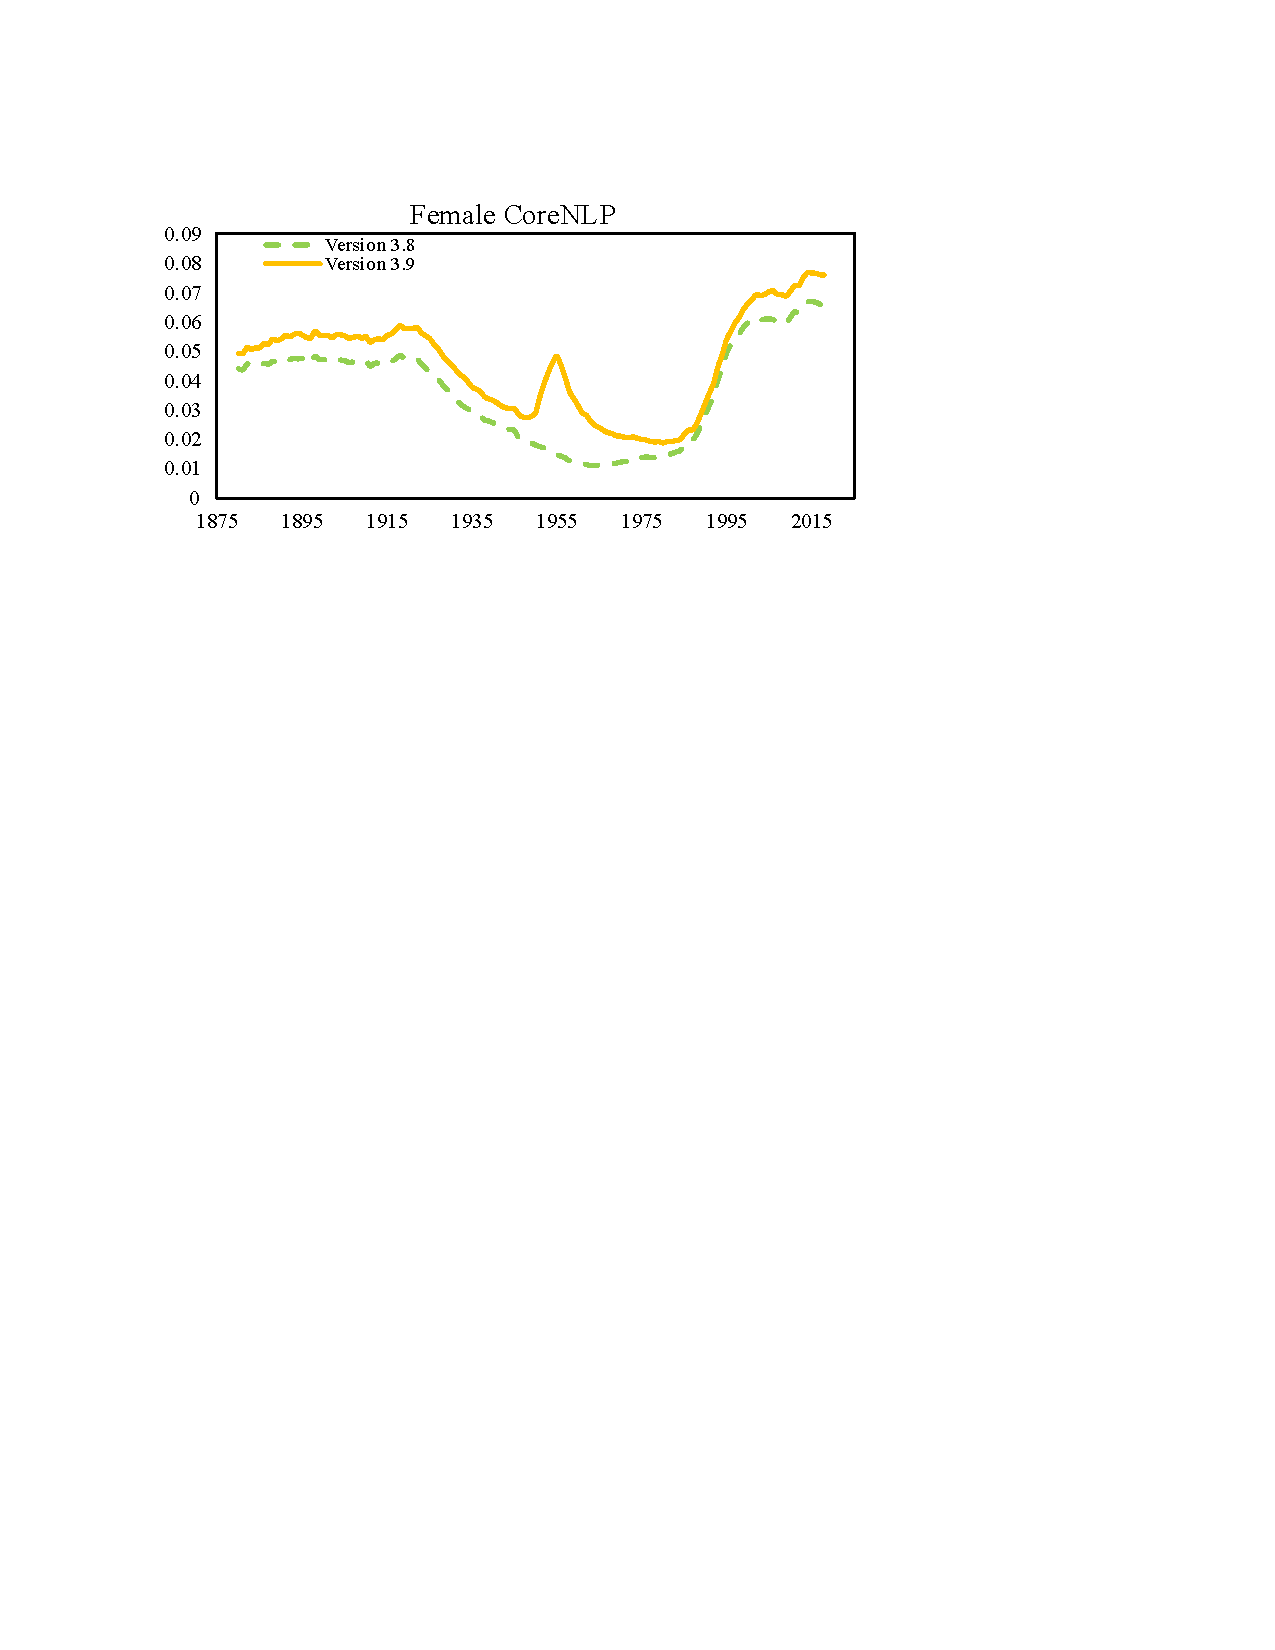
\includegraphics[width=\textwidth,height=0.55\textwidth,trim=0cm 0cm 0cm 0cm,clip=true]{images/corenlp_version_results/corenlp_version_1.pdf}
\end{subfigure}
\begin{subfigure}[b]{0.33\textwidth}
\caption{Error Type-3 Weighted}
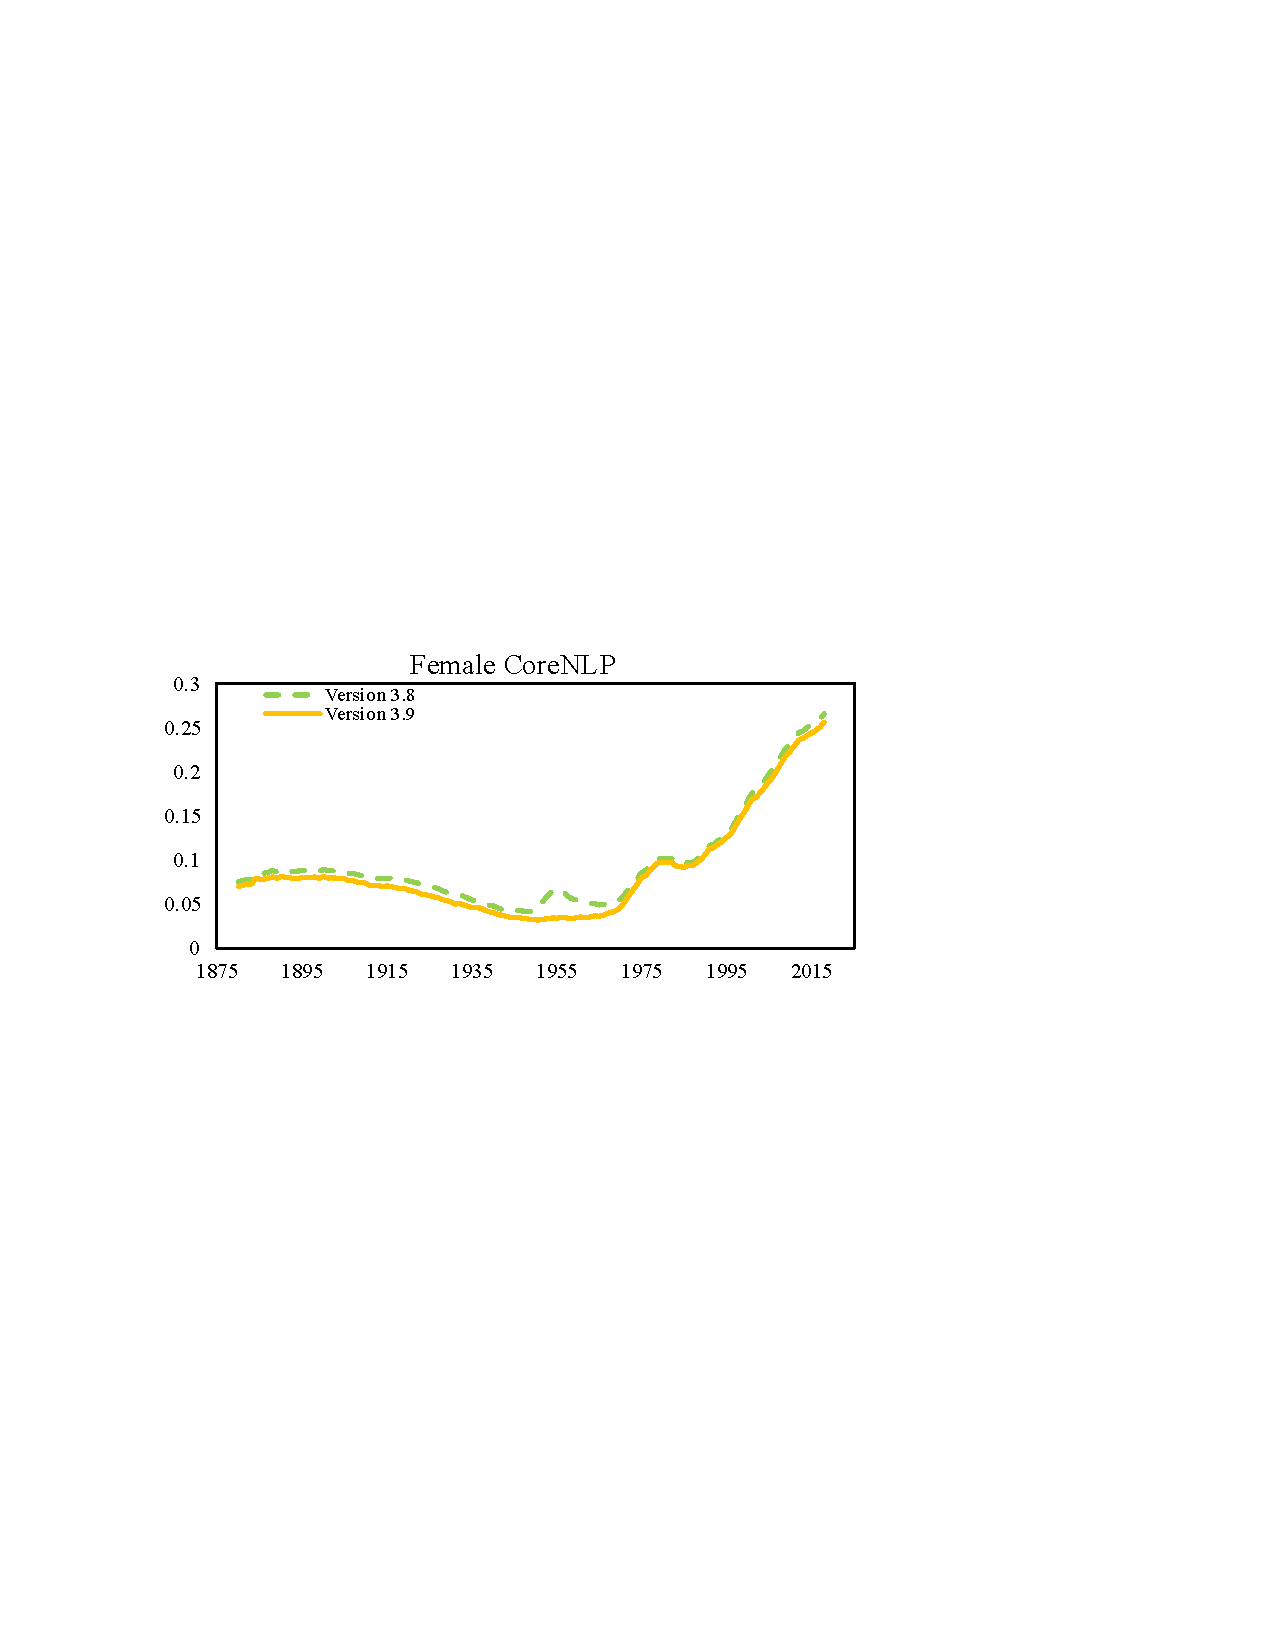
\includegraphics[width=\textwidth,height=0.55\textwidth,trim=0cm 0cm 0cm 0cm,clip=true]{images/corenlp_version_results/corenlp_version2.pdf}
\end{subfigure}
\begin{subfigure}[b]{0.33\textwidth}
\caption{Error Type-1 Weighted}
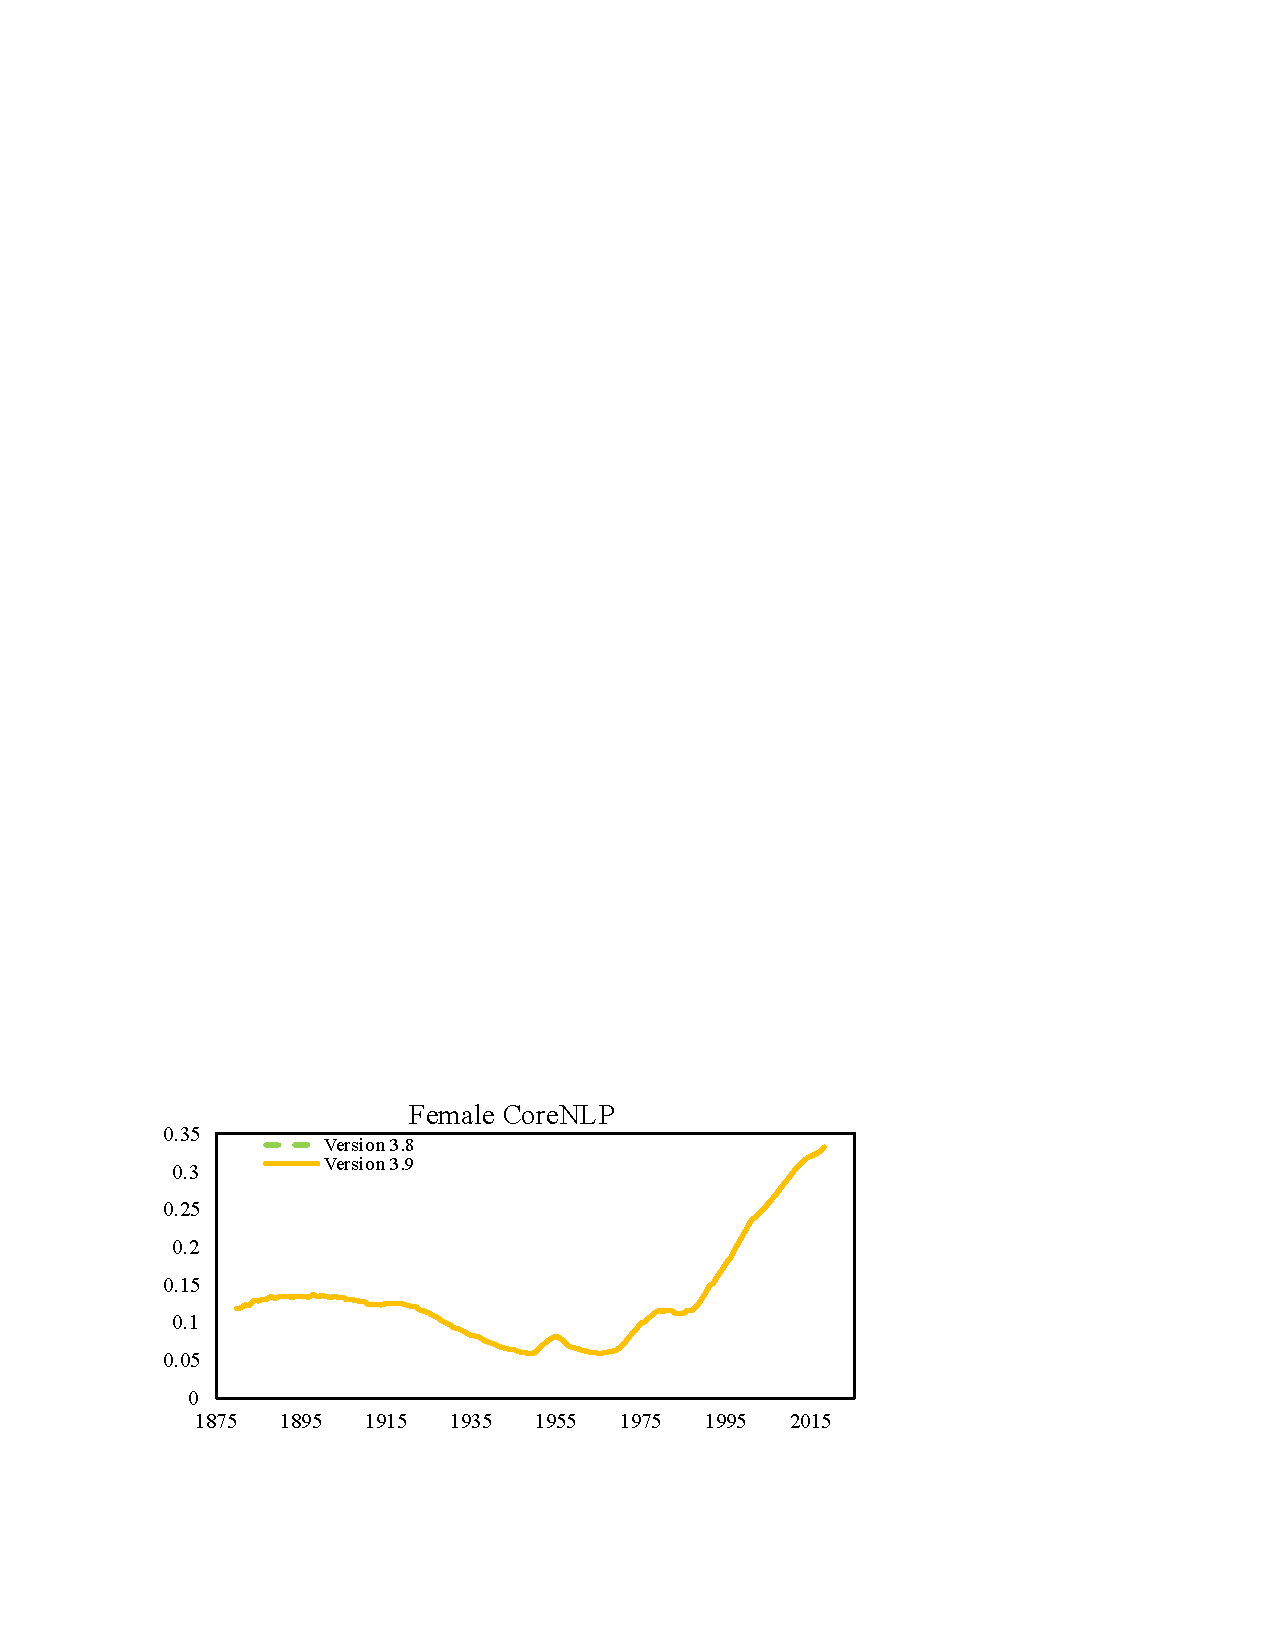
\includegraphics[width=\textwidth,height=0.55\textwidth,trim=0cm 0cm 0cm 0cm,clip=true]{images/corenlp_version_results/corenlp_version3.pdf}
\end{subfigure}
\begin{subfigure}[b]{0.33\textwidth}
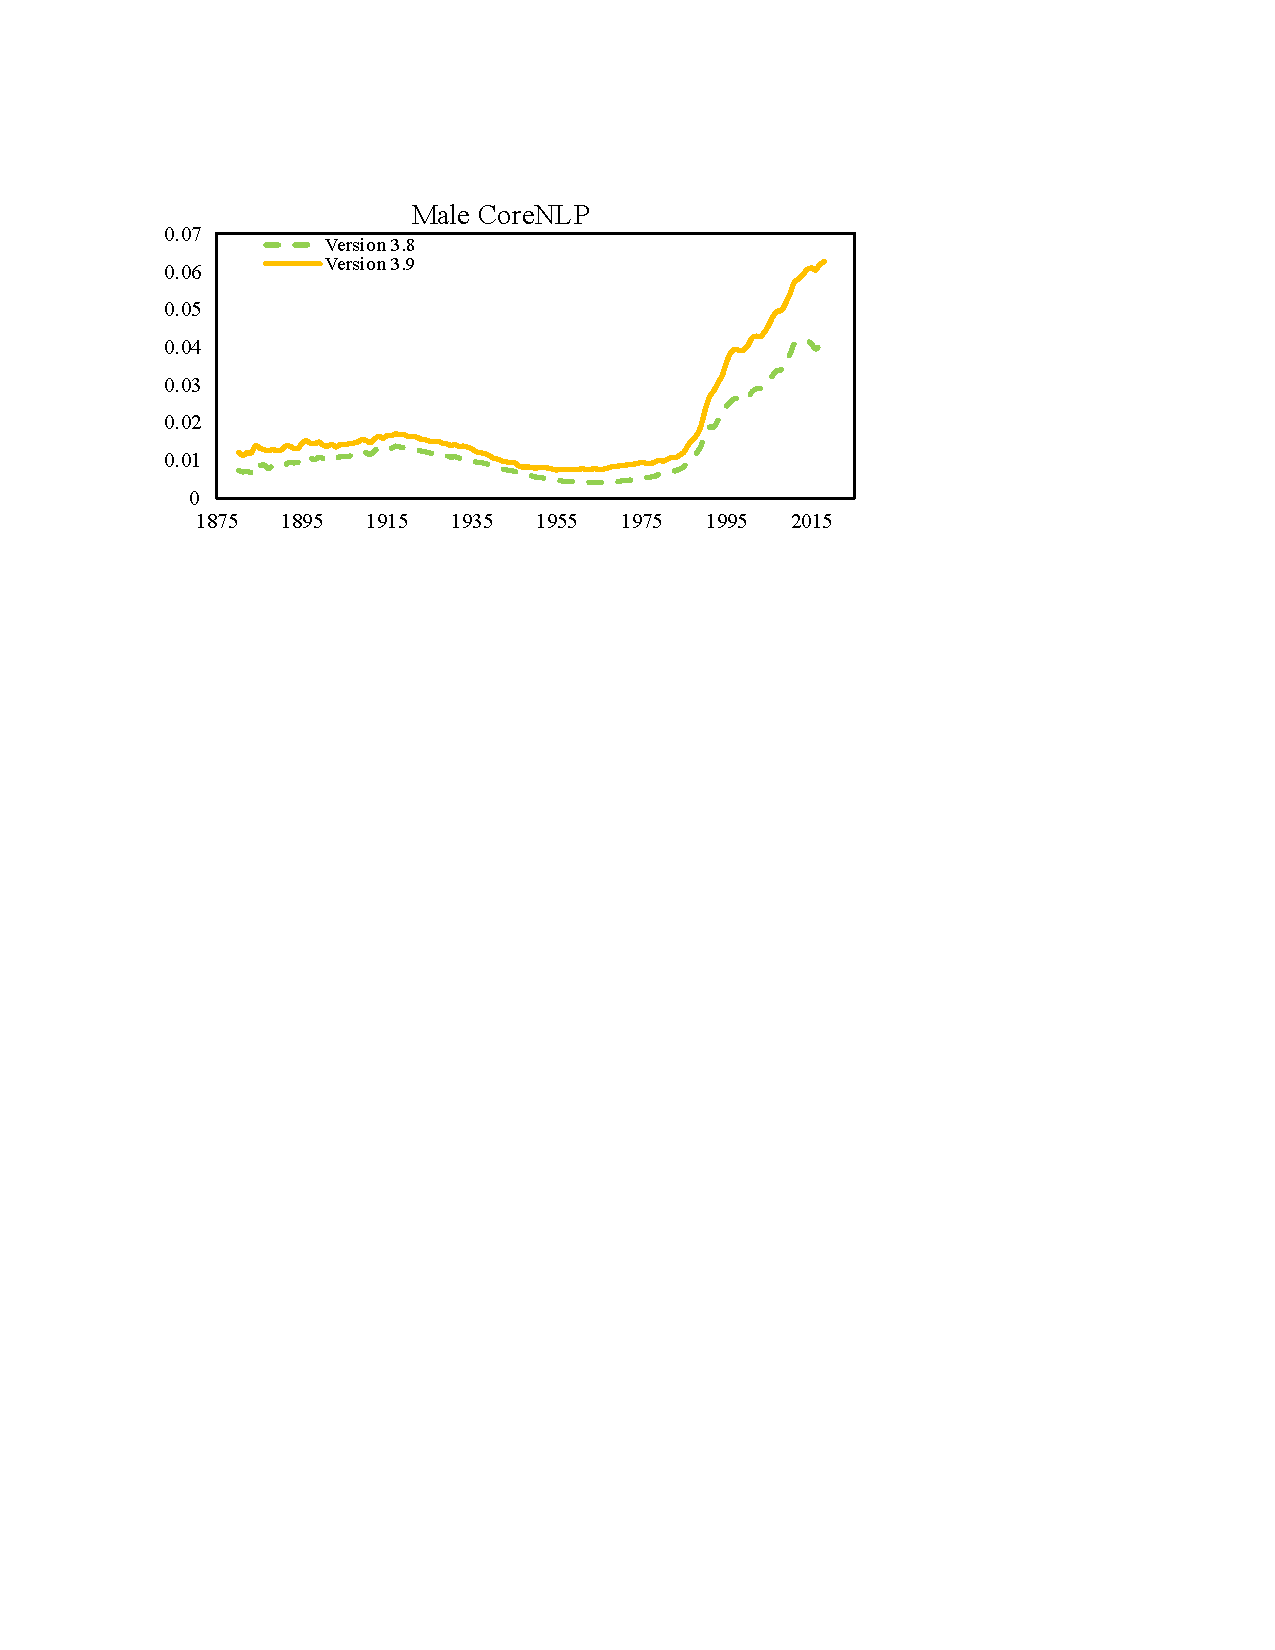
\includegraphics[width=\textwidth,height=0.55\textwidth,trim=0cm 0cm 0cm 0cm,clip=true]{images/corenlp_version_results/corenlp_version4.pdf}
\end{subfigure}
\begin{subfigure}[b]{0.33\textwidth}
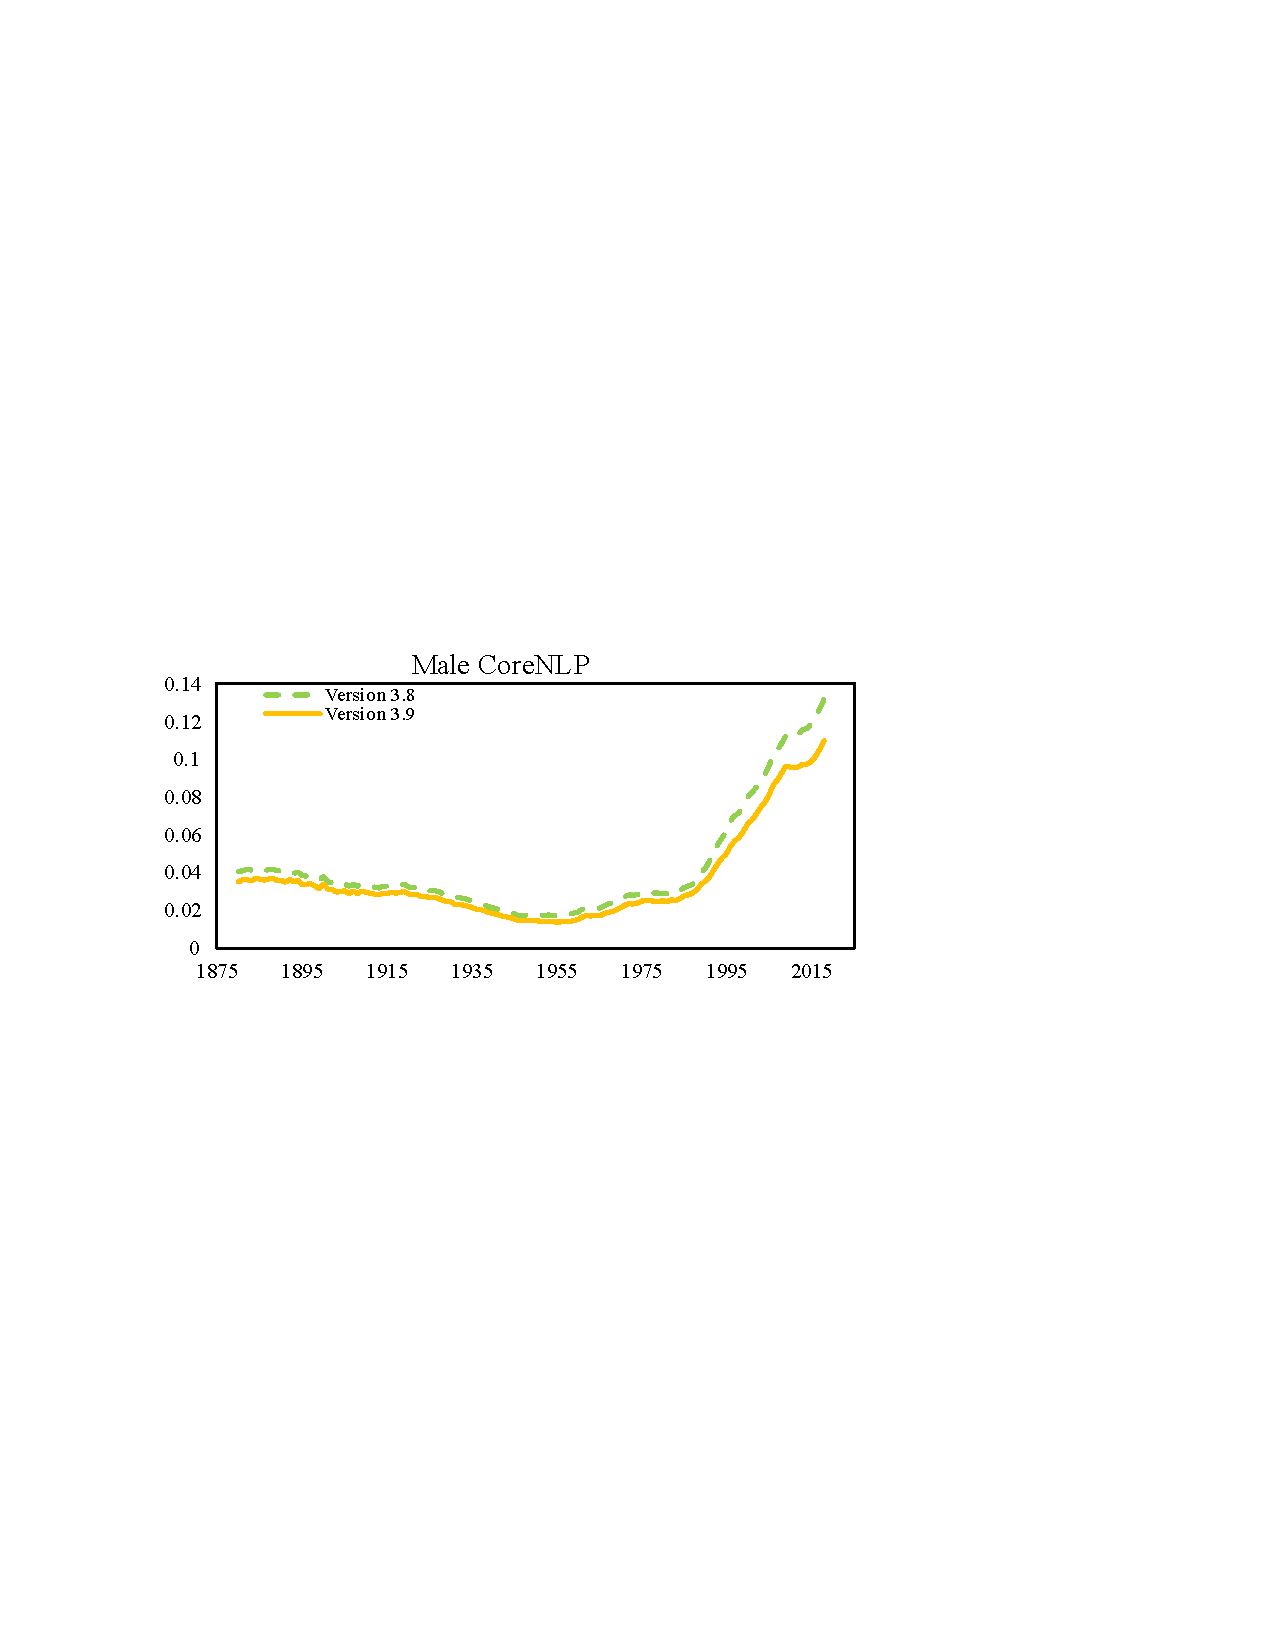
\includegraphics[width=\textwidth,height=0.55\textwidth,trim=0cm 0cm 0cm 0cm,clip=true]{images/corenlp_version_results/corenlp_version5.pdf}
\end{subfigure}
\begin{subfigure}[b]{0.33\textwidth}
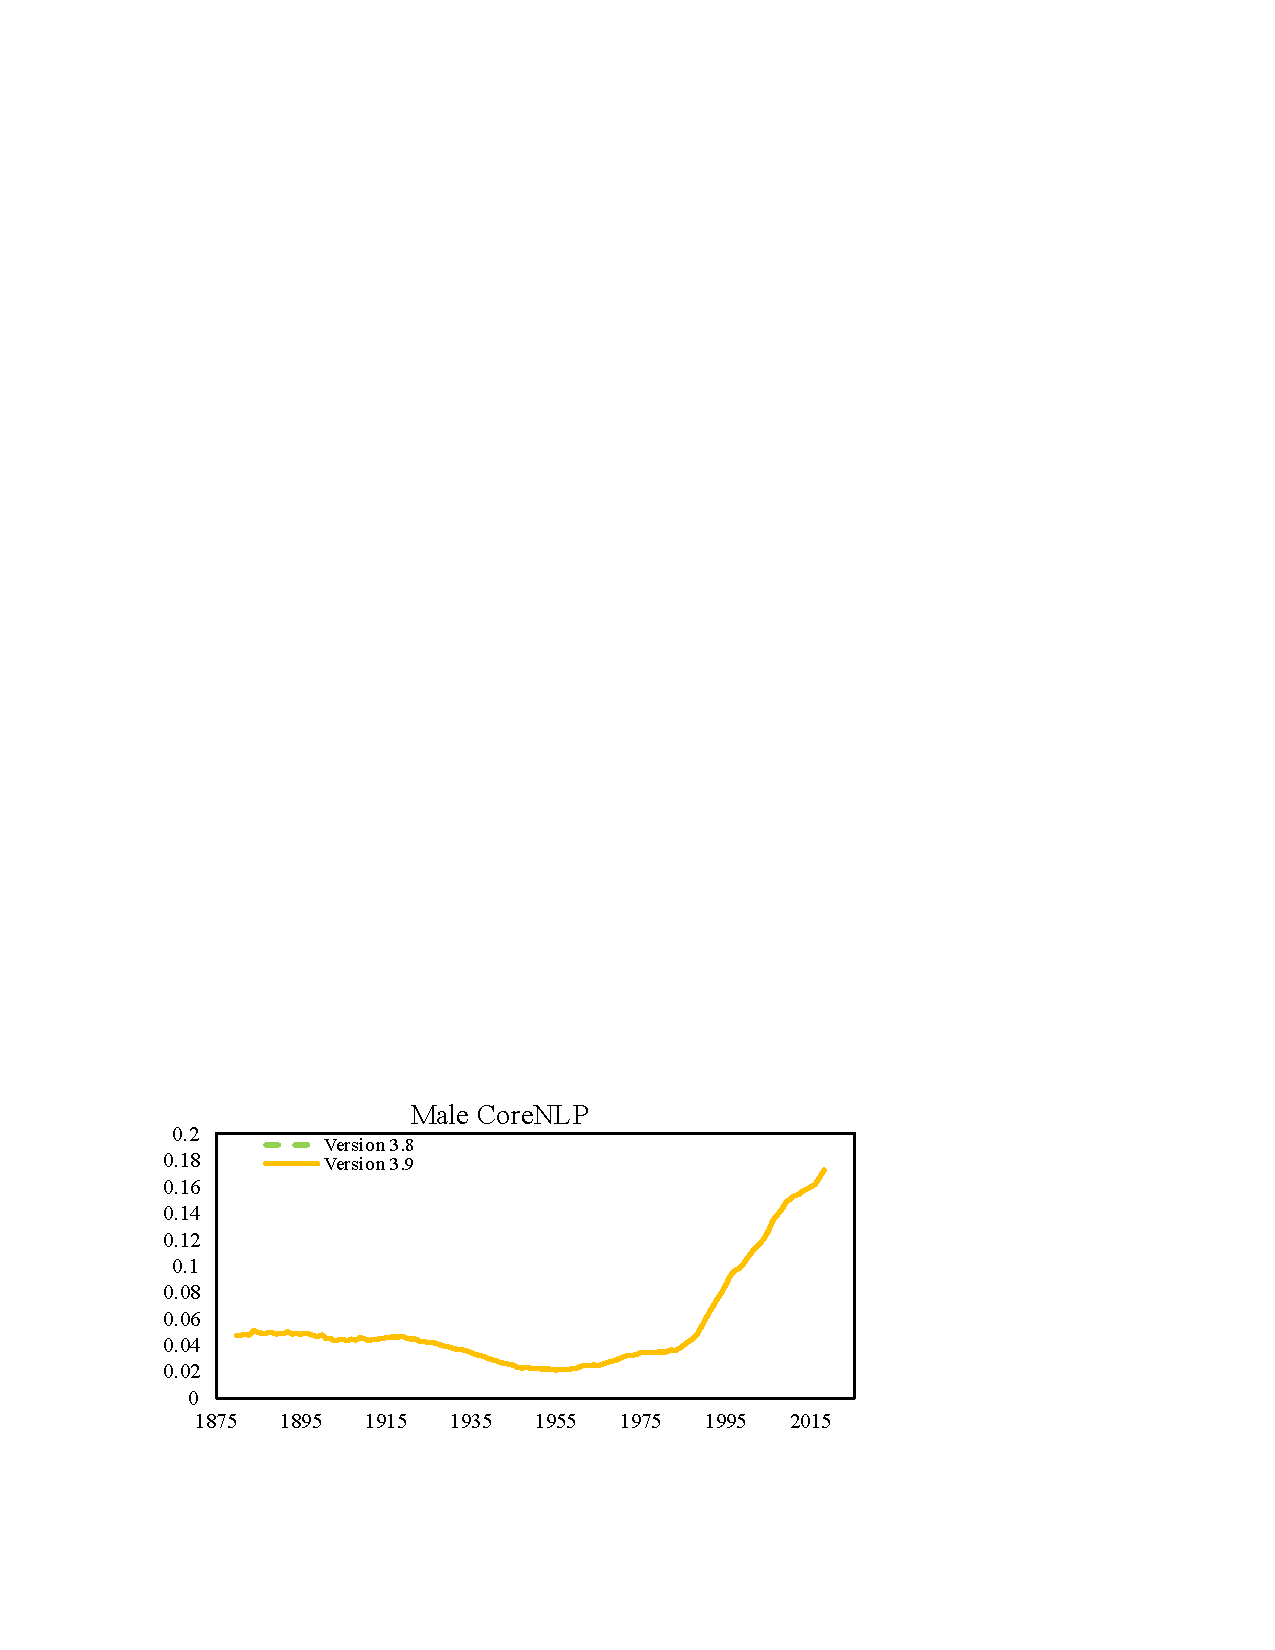
\includegraphics[width=\textwidth,height=0.55\textwidth,trim=0cm 0cm 0cm 0cm,clip=true]{images/corenlp_version_results/corenlp_version6.pdf}
\end{subfigure}
\caption{Version update in the CoreNLP model tried to tag more entities and thus a subtle boost in performance with regard to Error Type-3. However, this resulted in more PERSON entities being tagged as non-PERSON entities.  This then degraded performance with regard to Error Type-2 in the newer version, and overall no change in the Error Type-1 case which is considered to be the super-set. We observe how the degrade in Error Type-2 affected more female names than males on average.}
\label{corenlp_versions}
\end{figure*}
We used the train, test, and development sets from two widely known CoNLL-2003\footnote{\small{\url{https://www.clips.uantwerpen.be/conll2003/ner/}}} \cite{sang2003introduction} and OntoNotes-5\footnote{\small{\url{https://catalog.ldc.upenn.edu/LDC2013T19}}} \cite{weischedel2012ontonotes} datasets which were used in the training and testing of Flair, Spacy, and many other models. The split of the OntoNotes-5 dataset into train, development, and test sets was performed according to \cite{pradhan2013towards}. We reported the percentages of male vs. female names from the census data that appeared in train, test, and development sets in each of the datasets and compared this to the percentages of male vs. female names in reality from the census data to see how much these datasets are reflective of the reality or if they pertain to any bias toward a specific gender group.

Our results shown in Table \ref{data_stats_table} indicate that the datasets used do not reflect the real world, but rather exactly the opposite of that. Unlike the census data, which is representative of real-world statistics, wherein female names have more versatility---62\% unique names vs. 38\% unique male names---datasets used in training the NER models contain 42\% female names vs. 58\% male names from the census data. Not only do the datasets not contain more versatile female names to reflect the reality,  but instead have even less variety which can itself bias the models by not covering enough female names. Similar patterns are observable in test and development sets of datasets used in the NER systems.

